\chapter{作品设计与实现}

\section{系统方案}

\subsection{系统模型}
\begin{figure}[htbp]
    \centering
    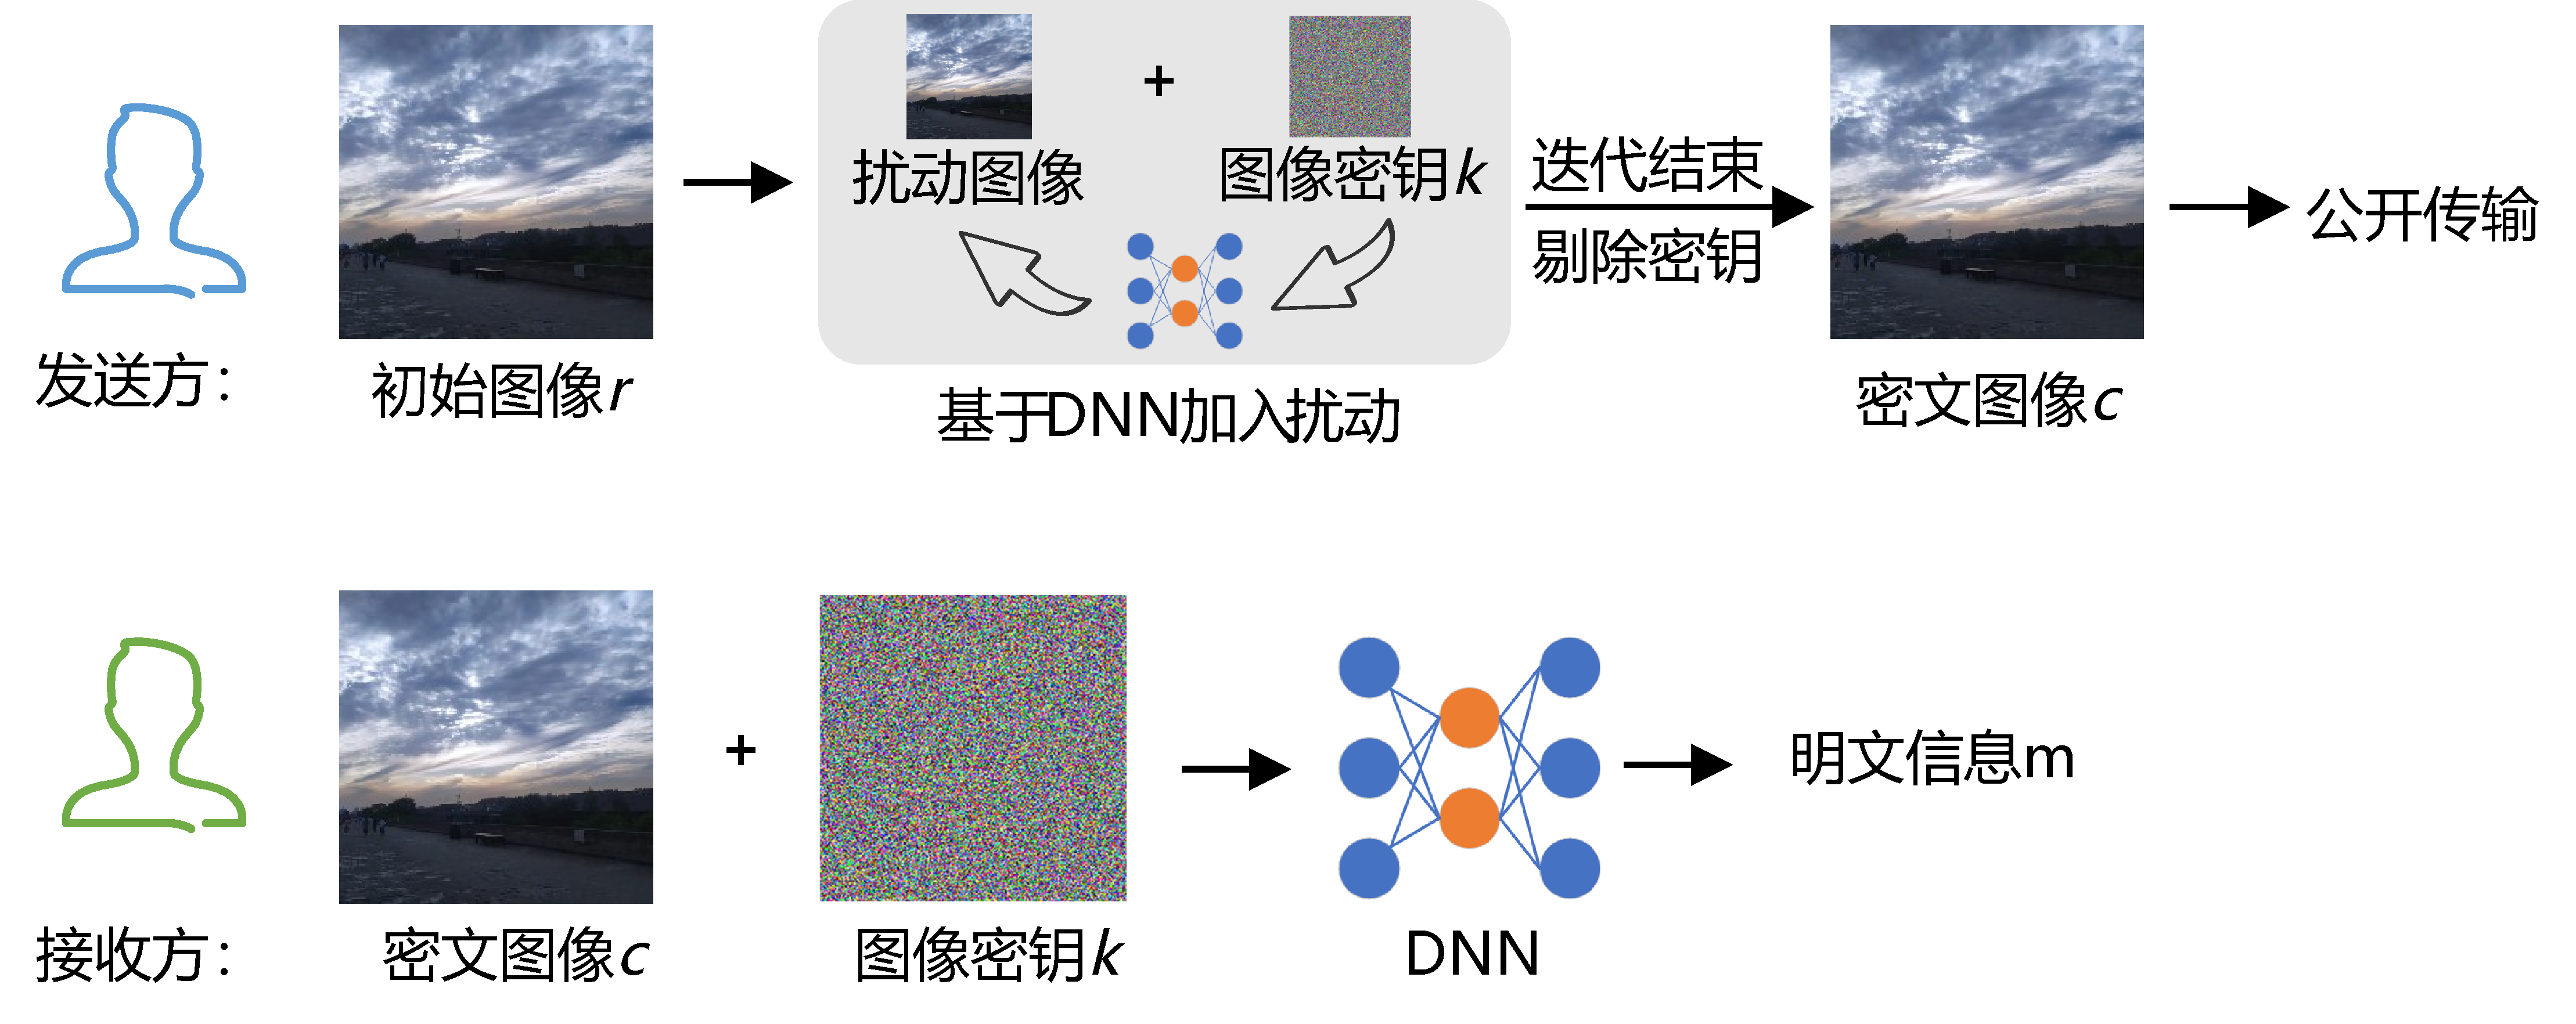
\includegraphics[width=\textwidth]{figures/fig-sys-model}
    \caption{SSIR 系统模型}
    \label{fig:sys-model}
\end{figure}

如图~\ref{fig:sys-model} 所示，SSIR 面向由发送方与接收方构成的两方通信场景。与传统直接对明文施加密码变换的“先加密、后解密”范式不同，SSIR 将待传输的消息映射为公开深度神经网络（DNN）在特定输入下呈现的内部神经元状态，并利用公开传输的密文图像与双方秘密共享的图像密钥之间的像素级叠加关系，实现受密钥控制的信息表示与恢复。在部署条件上，通信双方仅需具备基础计算能力，并配备结构与参数完全一致的公开预训练图像分类模型（如 ResNet~\cite{21-he-et-al-2016}、ShuffleNet V2~\cite{24-ma-et-al-2018}），无需引入可信第三方或专用硬件支持。

在实际通信前，收发双方通过安全信道预先共享一张图像密钥。当发送方需要传输明文消息时，首先将其编码为目标比特串，同时随机选取一张初始图像并与图像密钥逐像素叠加，构造出融合图像输入至 DNN 中，以观测选定神经元的激活响应。若当前神经元响应经编码后所得的比特串与目标比特串不符，发送方便利用 DNN 的梯度信息对扰动图像进行迭代微调，直至融合图像能够驱动 DNN 呈现出与明文消息完全对应的目标状态。微调收敛后，发送方从融合图像中减去图像密钥即可剥离出密文图像，并以无损格式经由公开信道发送。接收方作为合法通信实体，在收到密文图像后，只需将其与本地持有的同一图像密钥逐像素相加，即可还原出融合图像；随后将其输入同一 DNN 并读取相应神经元的响应，依据事先约定的分组编码规则即可直接解码出原始明文。由此可见，系统的计算开销主要集中在发送端的迭代优化阶段，而接收端的恢复过程仅包含一次图像加法与一次前向推理，无需任何迭代计算，因而具备极高的恢复效率。

在整个系统架构中，图像密钥是唯一需要保密的要素，而预训练 DNN 则作为公共计算资源被直接复用。图像密钥在形式上表现为与密文图像同尺寸的张量，其内容既可以是从特定分布中采样的随机噪声，也可以是任意自然图像，系统对其视觉语义不作限制。为消除跨平台计算误差，图像密钥、扰动图像、密文图像及模型输入均采用统一的固定精度张量格式进行存储与运算，以确保收发双方获得严格一致的数值结果。由于图像密钥通过逐像素加法参与融合图像的构造，且从未在公开信道中暴露，唯有持有正确密钥的接收方才能由密文图像还原出能够触发目标神经元状态的融合图像。与此同时，系统全程固定预训练 DNN 的公开参数，不对其进行重训练或微调，从而完整保留了模型原有的图像分类功能。正是因为深度神经网络具有高度非线性特征，同一图像密钥叠加在不同图像上所引起的神经元状态偏移与输入图像本身紧密耦合，从而奠定了图像密钥控制能力的安全基础；而网络自身的可微性质，则为发送端通过梯度反传开展对抗优化提供了计算支撑。

遵循 Kerckhoffs 原则，除上述图像密钥外，SSIR 所采用的模型结构与参数、编码规则、分组大小、二值化阈值以及优化超参数等配置均可完全公开。系统的安全性完全建立在图像密钥的保密性之上，攻击者即便掌握了完整的模型细节与编码机制，在缺乏图像密钥的情况下依然无法从公开截获的密文图像中提取出有效的明文信息。

\subsection{设计目标与阶段划分}
围绕上述通信模式，SSIR 在设计上致力于兼顾安全性、隐蔽性、运行效率与平台兼容性四方面要求。在安全层面，系统需保证未持有图像密钥的第三方无法恢复明文，在形式化意义下满足查询相关的选择明文安全（IND-CPA）与非自适应选择密文安全（IND-CCA1），能够有效抵御针对消息机密性与密钥保密性的各类分析攻击；在隐蔽层面，公开信道上传输的密文图像需尽可能抹除人为改动的痕迹，不仅要在视觉观感上与初始图像保持一致，还需确保攻击者在无密钥条件下将其直接输入 DNN 时，模型仅表现出与初始图像相近的常规状态；在效率与兼容性层面，系统应直接复用现有主流 DNN 架构而无需引入除图像密钥外的任何附加秘密，在完整保留宿主模型原有分类功能的前提下，支持紧凑型高价值消息的高效处理以及跨软硬件平台的稳定运行。

为实现上述目标，SSIR 的核心处理逻辑涵盖了消息编码、状态诱导、泄漏抑制优化以及消息恢复四个环节。顺应信息在系统中的流转次序，整体运行过程可划分为初始化、密文图像生成与消息恢复三个阶段。

在初始化阶段，通信双方完成密钥分发与公开参数的同步。双方运行密钥生成算法 \(k \leftarrow \mathrm{KeyGen}()\) 秘密生成并共享图像密钥，同时协商选定所使用的预训练 DNN 及配套的分组编码规范。该编码规范具体界定了用于承载消息的神经元所在网络层、选定神经元的索引顺序、每组相邻神经元的数量（即分组大小 \(g\)），以及将连续神经元激活值量化为二值比特的判别阈值 \(t \in (0,1)\)。

进入密文图像生成阶段后，发送方首先将待传明文 \(m\) 映射为目标比特串 \(S_t\)，并随机采样一张自然图像 \(r\)，经归一化与固定精度转换后作为初始扰动图像 \(p_0\)。在此基础上，发送方循环执行密钥叠加、前向推理、当前比特串编码、联合损失计算以及基于梯度的扰动更新操作。每完成一步更新，发送方便重新合成融合图像并检验当前解码所得比特串 \(S_c\) 是否与目标串 \(S_t\) 完全吻合；一旦两者一致即终止迭代，并从最终融合图像中减去图像密钥 \(k\)，输出密文图像 \(c\)。

在最后的消息恢复阶段，接收方将接收到的密文图像 \(c\) 与本地图像密钥 \(k\) 逐像素叠加，重构出融合图像 \(i\) 并送入 DNN 进行单次前向传播，读取目标神经元状态后按既定分组规则完成阈值判别与逆映射，即可无损还原出明文消息 \(m\)。

\section{实现原理}
本节结合系统核心处理环节，详细阐述 SSIR 的底层数学模型与实现机理，文中所涉主要符号及其定义汇总于表~\ref{tab:symbols}。

\begin{table}[htbp]
    \centering
    \caption{符号说明表}
    \label{tab:symbols}
    {\renewcommand{\arraystretch}{1.4}
    \begin{tabular}{cc}
        \hline
        符号 & 含义 \\
        \hline
        \(k\) & 图像密钥 \\
        \(m\) & 明文消息 \\
        \(S_t\)、\(S_c\) & 目标比特串、当前比特串 \\
        \(f_\theta\) & 所复用的深度神经网络 \\
        \(z(i)\) & 融合图像 \(i\) 在选定神经元上的连续状态向量 \\
        \(L_s=(ls_1,\dots,ls_d)\) & 状态向量，\(d\) 为选定神经元个数 \\
        \(g\) & 分组大小（每组相邻神经元个数） \\
        \(t\) & 编码阈值，\(t\in(0,1)\) \\
        \(\alpha\)、\(\beta\) & 直接/间接泄漏损失的权重 \\
        \(lr\) & 学习率（更新步长） \\
        \(\xi\) & 执行级随机状态 \\
        \(T_{\mathrm{trc}}\) & 截断操作 \\
        \(p_n\)、\(c\) & 扰动图像、密文图像 \\
        \(i_n\) & 融合图像 \\
        \(l_{\mathrm{be}}\)、\(l_d\)、\(l_{\mathrm{id}}\) & 位错误损失、直接泄漏损失、间接泄漏损失 \\
        \hline
    \end{tabular}}
\end{table}

在分组编码环节，系统需建立连续神经元激活值与离散消息比特之间的映射关系。发送方首先利用双射编码函数将明文消息 \(m\) 转化为长度为 \(\ell = \vert{}S_t\vert{}\) 的二进制目标比特串 \(S_t = \mathrm{Et}(m)\)。给定融合图像 \(i\)，DNN 在预设神经元集合上按既定顺序输出连续状态向量：
\begin{equation}
    L_s = (ls_1, ls_2, \ldots, ls_d) = z(i),
    \label{eq:state}
\end{equation}
其中 \(d\) 表示选定神经元的总数，\(ls_j\) 为第 \(j\) 个神经元的响应值。若直接以阈值 \(t\) 对单个神经元响应进行二值化，由于深度网络中常存在部分对输入微扰不够敏感的惰性神经元，其激活值在梯度优化中难以跨过预设阈值，极易造成个别比特编码失败并拖慢整体收敛。针对这一现象，SSIR 引入了分组编码机制：将相邻的 \(g\) 个神经元划分为一个编码组（满足 \(g \ell \le d\)），先求取组内神经元响应的算术平均值，再将该均值与阈值 \(t\) 进行比对，从而导出当前比特串 \(S_c = \mathrm{Ec}(z(i); g, t)\)。第 \(i\) 个比特 \(s_{c_i}\)（\(1 \le i \le \ell\)）的判定方式可表示为：
\begin{equation}
    s_{c_i} =
    \begin{cases}
        1, & \overline{ls}_i \ge t, \\
        0, & \overline{ls}_i < t,
    \end{cases}
    \qquad
    \overline{ls}_i = \frac{1}{g}\sum_{q=1}^{g} ls_{(i-1)g+q}
    \label{eq:encoding}
\end{equation}
这种组内均值池化策略有效降低了编码过程对单一神经元响应灵敏度的依赖。即便组内个别神经元响应迟钝，只要同组其余神经元在梯度引导下产生足够的补偿响应使组均值越过阈值，该比特位即可正确编码。该策略仅以单次表示容量由 \(d\) 缩减至 \(\lfloor d/g \rfloor\) 为代价，显著提升了状态诱导的收敛率与稳定性。

在分组编码的基础上，状态诱导旨在通过梯度优化求解出一幅特定扰动图像，使其与图像密钥叠加后能够驱动 DNN 产生与 \(S_t\) 一致的内部响应。发送方将随机采样的初始图像 \(r\) 归一化为初始扰动图像 \(p_0\)，并在第 \(n\) 轮迭代中将其与图像密钥 \(k\) 逐像素叠加构造融合图像 \(i_n\)：
\begin{equation}
    p_0 = \frac{r}{255}, \qquad i_n = p_n + k
    \label{eq:fusion}
\end{equation}
将 \(i_n\) 输入网络并完成分组编码后，若当前比特串 \(S_c\) 与目标串 \(S_t\) 尚不一致，则通过计算各组响应均值与目标比特之间的均方误差来度量位错误损失：
\begin{equation}
    l_{\mathrm{be}}^{(n)} = \sum_{i=1}^{\ell} \left( \overline{ls}_i^{(n)} - s_{t_i} \right)^2
    \label{eq:biterror}
\end{equation}
由于 \(l_{\mathrm{be}}^{(n)}\) 关于输入扰动图连续可微，发送方可通过反向传播求取其关于 \(p_n\) 的梯度并迭代修正像素值。需要指出的是，连续型损失 \(l_{\mathrm{be}}^{(n)}\) 仅用于提供梯度下降的搜索方向，而迭代终止则严格以离散条件 \(S_c = S_t\) 作为判据。当状态诱导收敛后，发送方从融合图像中剥离图像密钥即可获得最终的密文图像：
\begin{equation}
    c = i_n - k = p_n
    \label{eq:cipher}
\end{equation}
由此可见，公开传输的密文图像 \(c\) 本质上是经迭代优化后的扰动图像 \(p_n\)，其自身并不包含图像密钥 \(k\) 的成分，第三方仅凭观测 \(c\) 无法直接还原出能够触发目标神经元状态的融合图像。

然而，单纯追求状态诱导的达成可能会在扰动图像中留下异常痕迹：一方面，像素微调可能引起密文图像 \(p_n\) 与初始图像 \(p_0\) 之间的视觉失真，构成直接信息泄漏；另一方面，攻击者即便没有密钥，也可将截获的 \(p_n\) 直接送入公开 DNN 中，通过比对模型内部响应的异常波动来实施检测或分析，从而构成间接信息泄漏。为同步抑制上述两类风险，SSIR 在优化目标中引入了双重泄漏约束。其中，直接信息泄漏损失利用预训练视觉特征提取网络 \(\mathrm{vgg}\) 度量 \(p_n\) 与 \(p_0\) 在感知特征空间的偏离程度：
\begin{equation}
    l_d^{(n)} = \left| \mathrm{vgg}(p_n) - \mathrm{vgg}(p_0) \right|
    \label{eq:leak-direct}
\end{equation}
间接信息泄漏损失则用于约束无密钥条件下 \(p_n\) 与 \(p_0\) 在宿主模型 \(f_\theta\) 选定特征表示层 \(R\) 上的响应差异：
\begin{equation}
    l_{\mathrm{id}}^{(n)} = \left| R(f_\theta(p_n)) - R(f_\theta(p_0)) \right|
    \label{eq:leak-indirect}
\end{equation}
此外，考虑到不同硬件设备（如不同架构的 GPU 与 CPU）在底层浮点数运算上存在微小舍入差异，处于阈值边界附近的神经元状态可能因跨设备推理而发生比特翻转。同时为了保证生成的密文图像符合标准无损图像格式要求，系统在每步梯度更新后均对扰动图像施加截断操作 \(T_{\mathrm{trc}}\)，即先将像素值裁剪至 \([0,1]\) 区间，再按 8 位色深阶梯进行离散化量化并以 32 位浮点格式（float32）存储：
\begin{equation}
    T_{\mathrm{trc}}(x) = \frac{\lfloor 255x \rfloor}{255}, \quad x \in [0,1]
    \label{eq:trunc}
\end{equation}
此处截断与裁剪仅作用于扰动分量 \(p_n\)，而融合图像 \(i_n = p_n + k\) 的合成则严格执行逐元素可交换加法，不对其进行额外的数值裁剪，从而避免引入非线性截断误差。综合位错误损失与两项泄漏约束，第 \(n\) 轮迭代的联合损失函数及扰动图像更新规则可表述为：
\begin{equation}
    L^{(n)} = l_{\mathrm{be}}^{(n)} + \alpha l_d^{(n)} + \beta l_{\mathrm{id}}^{(n)}
    \label{eq:jointloss}
\end{equation}
\begin{equation}
    p_{n+1} = T_{\mathrm{trc}} \left( \mathrm{R\text{-}FGSM} \left( p_n, \nabla_{p_n} L^{(n)}, lr; \xi, n \right) \right)
    \label{eq:update}
\end{equation}
式中，\(\alpha\) 与 \(\beta\) 分别为两项泄漏损失的平衡权重，\(lr\) 为更新步长。系统采用随机化快速梯度符号法（R-FGSM）沿梯度符号方向执行带随机扰动的一步更新，其步长扰动行为由每次执行时独立采样的随机状态 \(\xi\) 控制。每次加密时独立选取的初始图像 \(r\) 与执行级随机状态 \(\xi\) 共同构成了系统的两级随机源，赋予密文生成过程概率化特征，以满足密码学语义安全要求。在联合优化过程中，\(l_{\mathrm{be}}^{(n)}\) 驱动叠加密钥后的融合图像逼近目标编码状态，而 \(l_d^{(n)}\) 与 \(l_{\mathrm{id}}^{(n)}\) 则将无密钥下的密文图像锚定在初始图像附近。权衡系数 \(\alpha\)、\(\beta\) 及步长 \(lr\) 均由发送方在本地自主设定，接收方在解码时无需获知上述超参数。

当密文图像 \(c\) 传输至接收端后，消息恢复过程作为生成的逆向映射即可直接展开。接收方将密文图像 \(c\) 与本地图像密钥 \(k\) 逐像素相加重构融合图像 \(i\)，经 DNN 前向推理提取选定神经元状态后，依次执行分组阈值解码与双射逆变换 \(\mathrm{Et}^{-1}\)：
\begin{equation}
    i = c + k, \qquad S_t = \mathrm{Ec}(z(i); g, t), \qquad m = \mathrm{Et}^{-1}(S_t)
    \label{eq:recover}
\end{equation}
得益于逐像素加法的交换律以及收发双方统一的固定数值精度，接收端合成的融合图像 \(i = c + k = p_n + k\) 与发送端终止迭代时的融合图像完全等同，因此在同一确定性 DNN 映射下必然产出一致的神经元状态，从而确保明文消息的精确恢复。

\section{系统流程}
在明确底层原理的基础上，图~\ref{fig:lifecycle} 展示了 SSIR 从参数协商到消息还原的完整运行生命周期。通信双方在初始化阶段完成图像密钥共享与编码配置同步后，即可持续开展保密通信：发送方在本地完成迭代式的密文图像生成，并将结果以无损图像格式投入公开信道；接收方获取图像后通过单次前向推理完成确定性解码。这种非对称的计算负载分配使得复杂的对抗优化完全由发送方承担，极大减轻了接收方的实时处理负担。

\begin{figure}[htbp]
    \centering
    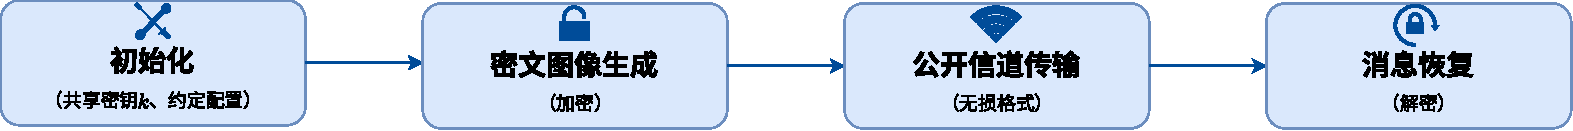
\includegraphics[width=\textwidth]{figures/fig-lifecycle}
    \caption{系统生命周期}
    \label{fig:lifecycle}
\end{figure}

发送端生成密文图像的具体执行逻辑如图~\ref{fig:gen-flow} 与算法~\ref{alg:gen} 所示。算法以随机初始图像 \(r\)、执行级随机状态 \(\xi\)、明文 \(m\) 及共享图像密钥 \(k\) 等作为输入。初始化完成后，发送方在 `while` 循环中持续检验当前融合图像 \(p_n+k\) 所触发的编码比特串是否已收敛至目标串 \(S_t\)。只要两者存在偏差，算法便计算包含位错误损失、直接泄漏损失与间接泄漏损失的联合目标函数 \(L^{(n)}\)，并调用结合了固定精度截断算子 \(T_{\mathrm{trc}}\) 的 R-FGSM 规则更新扰动图像 \(p_{n+1}\)。一旦某轮迭代后满足 \(\mathrm{Ec}(z(p_n+k); g, t) = S_t\)，循环立即终止，此时的扰动图像 \(p_n\) 即作为密文图像 \(c\) 输出。

\begin{figure}[htbp]
    \centering
    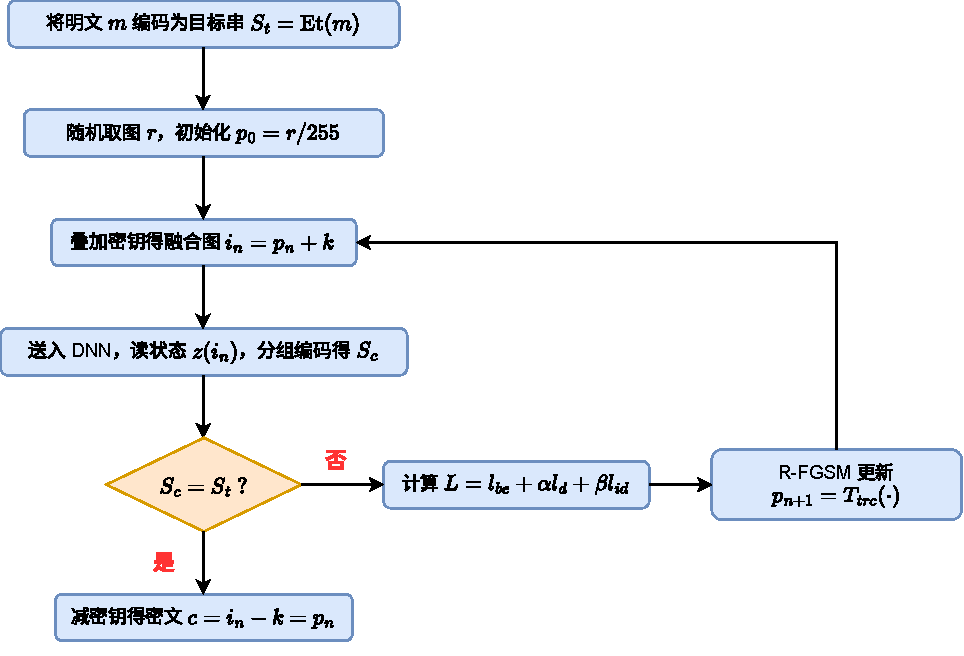
\includegraphics[width=\textwidth]{figures/fig-gen-flow}
    \caption{密文图像生成流程}
    \label{fig:gen-flow}
\end{figure}

\begin{algorithm}[htbp]
    \caption{密文图像生成}
    \label{alg:gen}
    \begin{algorithmic}[1]
        \Require 随机图像 \(r\)，随机状态 \(\xi\)，明文消息 \(m\)，图像密钥 \(k\)，DNN \(f_\theta\)，状态读出 \(z\)，编码函数 \(\mathrm{Et}\)、\(\mathrm{Ec}\)，以及参数 \(g\)、\(t\)、\(\alpha\)、\(\beta\)、\(lr\)、\(T_{\mathrm{trc}}\)
        \Ensure 密文图像 \(c\)
        \State \(p_0 \leftarrow r/255\)，\(S_t \leftarrow \mathrm{Et}(m)\)，\(n \leftarrow 0\)
        \While{\(\mathrm{Ec}(z(p_n+k); g, t) \neq S_t\)}
            \State \(i_n \leftarrow p_n + k\)
            \State \(L^{(n)} \leftarrow l_{\mathrm{be}}^{(n)} + \alpha l_d^{(n)} + \beta l_{\mathrm{id}}^{(n)}\)
            \State \(p_{n+1} \leftarrow T_{\mathrm{trc}}\left(\mathrm{R\text{-}FGSM}(p_n, \nabla_{p_n} L^{(n)}, lr; \xi, n)\right)\)
            \State \(n \leftarrow n + 1\)
        \EndWhile
        \State \(c \leftarrow p_n\)
        \State \Return \(c\)
    \end{algorithmic}
\end{algorithm}

相对应地，接收端的消息恢复流程如图~\ref{fig:recover-flow} 所示。接收方将密文图像与本地图像密钥逐像素叠加后送入 DNN，提取目标层选定神经元的激活状态，经分组均值计算与阈值二值化还原出目标比特串，最后通过逆编码映射恢复出明文消息。整个恢复链路均为确定性张量运算，不涉及任何随机采样或梯度迭代。

\begin{figure}[htbp]
    \centering
    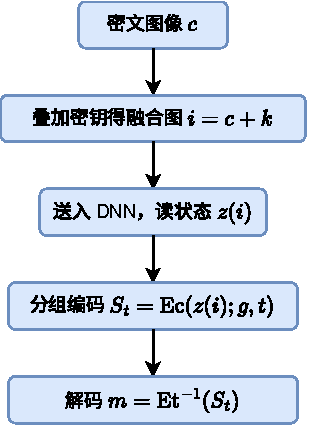
\includegraphics[width=0.4\textwidth]{figures/fig-recover-flow}
    \caption{消息恢复流程}
    \label{fig:recover-flow}
\end{figure}

\section{功能模块}
依据上述系统架构与运行流程，SSIR 在软件实现上解耦为密钥与配置管理、编码、状态诱导、泄漏抑制以及密钥叠加与恢复五个核心功能模块，各模块间的调用与协作关系如图~\ref{fig:modules} 所示。

\begin{figure}[htbp]
    \centering
    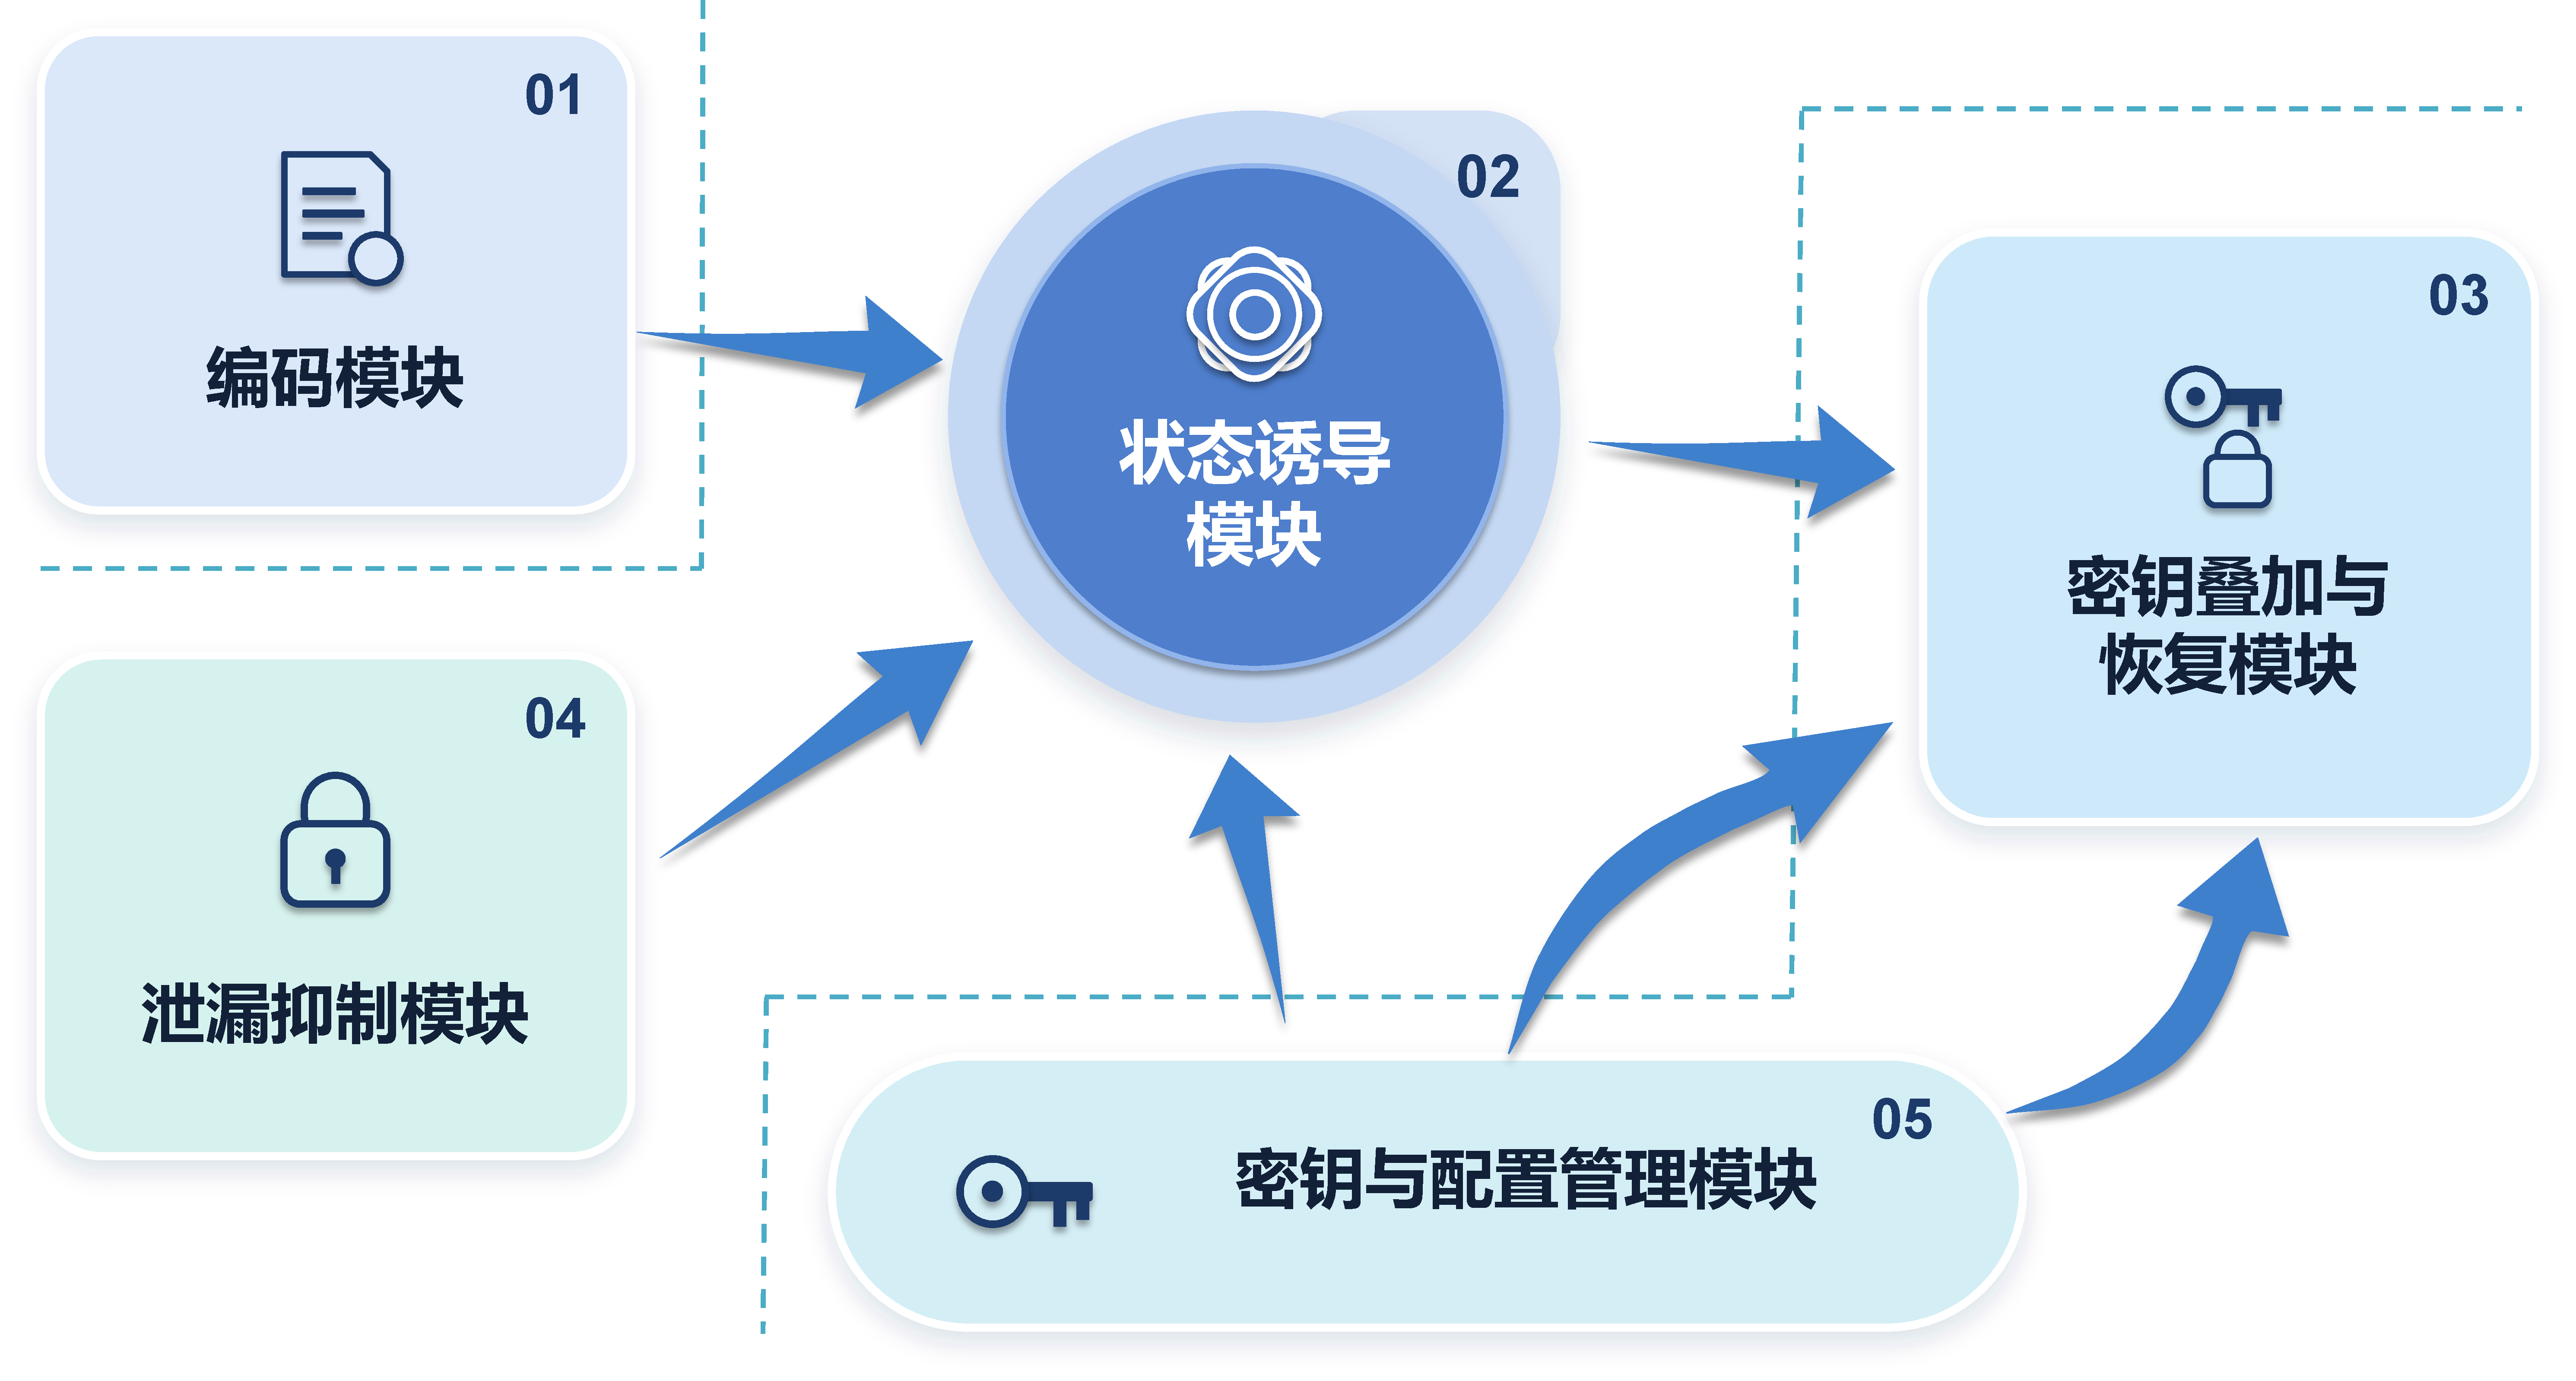
\includegraphics[width=\textwidth]{figures/fig-modules}
    \caption{系统功能模块}
    \label{fig:modules}
\end{figure}

其中，\textbf{密钥与配置管理模块}承担系统底层的运行支撑职责，负责图像密钥的生成、安全预共享与定期更新策略，并维护收发双方在宿主 DNN 架构、目标神经元位置及分组参数等方面的配置同步，确保两端处于严格一致的运行环境。\textbf{编码模块}在明文语义空间与神经元状态空间之间提供双向转换接口：在发送端负责将明文转化为目标比特串，并将每次推理所得的选定神经元连续状态按分组均值规则量化为当前比特串；在接收端则依据完全对称的规则将神经元状态逆向解码为明文消息。

在发送端的核心优化链路中，\textbf{状态诱导模块}与\textbf{泄漏抑制模块}紧密协同。状态诱导模块主导对抗优化循环，利用反向传播获取的梯度信息持续调整扰动图像，直至叠加图像密钥后的融合图像能够准确触发目标神经元状态；泄漏抑制模块则在每步梯度计算中嵌入基于视觉特征的直接泄漏损失与基于模型内部表征的间接泄漏损失，同时在像素更新后执行固定精度截断操作，以确保生成的密文图像兼具视觉隐蔽性、表征隐蔽性与跨平台数值鲁棒性。而在接收端，\textbf{密钥叠加与恢复模块}负责将接收到的密文图像与本地图像密钥逐像素合成，并调用宿主模型与编码模块完成单次前向推理与消息还原。

\section{性能指标}
综合实验测试与理论分析结果，SSIR 在安全性、隐蔽性、运行效率与架构兼容性四个方面均表现出良好的综合性能。在\textbf{安全性}方面，合法接收方在持有正确图像密钥时，消息恢复误码率稳定为 0\%，精确恢复率达 100\%；而在无密钥、随机伪造密钥或错误密钥条件下，攻击者解码所得比特串的误码率均维持在 50\% 左右，退化为完全随机猜测。与此同时，形式化安全证明给出了系统在查询相关 IND-CPA 与 IND-CCA1 威胁模型下的优势上界，支持用户根据目标安全预算灵活设定单密钥允许的最大生成与恢复查询次数。

在\textbf{隐蔽性}方面，密文图像与初始自然图像在视觉上高度吻合，峰值信噪比（PSNR）最高可达 41.93~dB，结构相似性（SSIM）达到 97.99\%；在泄漏抑制机制的作用下，直接信息泄漏指标低至 0.08，无密钥推理下的间接信息泄漏相较无约束基线平均降低了 56.02\%。在\textbf{运行效率与兼容性}方面，系统无需任何前期的模型训练或额外参数存储，准备开销为零；针对 150 位长度的消息，发送端生成一张密文图像仅耗时约 300--500~ms，接收端完成消息恢复仅需约 10~ms。此外，依托固定精度截断机制，系统在跨设备（GPU 与 CPU 混合部署）场景下的恢复误码率同样保持为 0\%，并且广泛兼容传统 CNN、Inception、Residual/Dense、Mobile/Efficient 以及注意力机制（Attention）等主流深度神经网络家族，在实现可靠信息传输的同时完整保留了宿主模型原有的业务功能。
